\documentclass[12pt]{article}

\usepackage{sbc-template}
\usepackage{graphicx,url}
\usepackage{subcaption}
\usepackage[utf8]{inputenc}
\usepackage[brazil]{babel}

     
\sloppy

\title{Análise Comparativa de Desempenho em Drivers para MongoDB em Aplicações Node.js}

\author{Leandro Ungari Cayres, Ronaldo Celso Messias Correia }


\address{Faculdade de Ciências e Tecnologia -- Universidade Estadual Paulista (UNESP)\\
  Presidente Prudente -- SP -- Brazil
  \email{\{leandro.ungari,ronaldo.correia\}@unesp.br}
}

\begin{document} 

\maketitle

\begin{abstract}
  This meta-paper describes the style to be used in articles and short papers
  for SBC conferences. For papers in English, you should add just an abstract
  while for the papers in Portuguese, we also ask for an abstract in
  Portuguese (``resumo''). In both cases, abstracts should not have more than
  10 lines and must be in the first page of the paper.
\end{abstract}
     
\begin{resumo} 
  Este meta-artigo descreve o estilo a ser usado na confecção de artigos e
  resumos de artigos para publicação nos anais das conferências organizadas
  pela SBC. É solicitada a escrita de resumo e abstract apenas para os artigos
  escritos em português. Artigos em inglês deverão apresentar apenas abstract.
  Nos dois casos, o autor deve tomar cuidado para que o resumo (e o abstract)
  não ultrapassem 10 linhas cada, sendo que ambos devem estar na primeira
  página do artigo.
\end{resumo}


\section{Introdução}
Nos últimos anos, o crescimento no volume de dados mudou a utilização desses por empresas e organizações; tais dados, inicialmente considerados agentes passivos, relacionados às regras de negócio empresarial; tornaram-se potenciais oportunidades de lucro através da análise de informações, e consequentemente, do conhecimento presente no conjunto de dados.

Essa crescente quantidade de dados, chamado de~\emph{Big Data}, não somente requer maior espaço de armazenamento, mas uma mudança em sua organização com base em cada contexto, considerando características como volume, variedade, velocidade e valores~\cite{ward2013undefined}.
A arquitetura dos tradicionais bancos de dados relacionais, baseada no modelo ACID (\textit{atomicity},~\textit{consistency},~\textit{isolation} e~\textit{durability}), contudo, em ambientes de~\emph{Big Data}, a alta consistência afeta diretamente os aspectos de disponibilidade e  eficiência, que são importantes, devido ao alto volume, variedade e velocidade presente em Big Data~\cite{aparicio:2016}. 

Nesse cenário surgem os banco de dados NoSQL (``Not only SQL'') provendo maior flexibilidade estrutural, suporte a replicação e consistência eventual consistência seguindo o critério BASE (\textit{basic},~\textit{availability},~\textit{soft-state} e~\textit{eventual consistency})~\cite{han2011survey}. 
Nos últimos anos, a popularidade dos banco de dados não-relacionais tem crescido~\cite{cooper2010benchmarking,edlich2015nosql} proporcionando diversas soluções conforme características dos dados cada aplicação.

Diferentemente do modelo relacional, os bancos NoSQL não possuem uma linguagem comum entre eles que permita a realização de operações, como o SQL (\emph{Structured Query Language}), desse modo, cada banco provê uma interface nativa para manipulação dos dados. 
Contudo, uso de chamadas de sistema para execução de comandos dessas interfaces não é reconhecida como uma boa prática, que pode incorrer em diversos problemas. 

De modo a contornar essa situação, para os diferentes ambientes de desenvolvimento e linguagens de programação,~\emph{drivers} tem sido desenvolvidos de modo a viabilizar a execução dos comandos no banco de dados. 
Em muitas situações, a decisão de qual combinação entre banco de dados não-relacional e~\emph{driver} a ser empregada pode ser um problema, devido a variedade de possibilidades, assim como o desconhecimento dos pontos positivos e negativos de cada solução.

Neste artigo, por meio de um estudo comparativo, busca-se avaliar as duas principais soluções de~\emph{drivers} para o MongoDB~\footnote{https://www.mongodb.com/}, respectivamente MongoClient~\footnote{https://mongodb.github.io/node-mongodb-native/} e Mongoose~\footnote{https://mongoosejs.com/}, em ambientes de aplicação Node.js. 
O principal fator considerado para a realização desse análise consiste na definição prévia de esquema para a manipulação dos dados em operações de CRUD (\emph{create}-\emph{read}-\emph{update}-\emph{delete}). Conceitualmente, os banco de dados não-relacionais não requerem esse predefinição, proporcionando flexibilidade, contudo não existe nada que impeça sua utilização, principalmente quanto a respeito do desempenho; possibilitando algum impacto relevante.

A escolha do banco de dados MongoDB ocorreu devido a sua enorme popularidade recente, empregado em diversas aplicações e linhas de pesquisa; o qual consiste na principal opção dentre os bancos de dados que adotam a estratégia de armazenamento orientada a documentos.
A respeito do ambiente Node.js, apesar de uma tecnologia recentes alguns trabalhos apontam a sua viabilidade no desenvolvimento de aplicações~\cite{chaniotis2015node}; além disso, com essa escolha, tanto aplicação quanto banco de dados utilizam JavaScript, permitindo a elaboração de um sistema uniforme, em termos de linguagem de programação.

Na análise conduzida neste trabalho, o desempenho do banco de dados MongoDB atrelado a cada um dos~\emph{drivers} investigados é analisado sobre perspectivas de tempo de execução, tempo de uso de processamento e consumo de memória sob um conjunto de dados genérico, propiciando a identificação de algumas características.

O restante desse trabalho está organizado do seguinte modo: na Seção~\ref{section:nao-relacional} é realiza uma revisão conceitual sobre banco de dados não-relacional, assim como sobre o MongoDB e seus drivers. A Seção~\ref{section:estudo} é apresentado o estudo comparativo realizado neste trabalho. Seção~\ref{section:resultados} são apresentados os resultados quantitativos obtidos, cuja discussão é elaborada na Seção~\ref{section:discussao}. Em seguida, na Seção~\ref{section:limitacoes} e, por fim, na Seção~\ref{section:consideracoes} as considerações finais desse trabalho.


\section{Banco de Dados Não-Relacional}
\label{section:nao-relacional}

Os bancos de dados NoSQL, "Não apenas SQL", foram desenvolvidos visando armazenar e processar grandes volumes de dados. Em linhas gerais os bancos de dados NoSQL são livres de esquematizações, lidam com dados não estruturados como e-mail, documentos e mídias sociais de maneira eficiente~\cite{mohamed:2014,ramesh:2016}.

O termo NoSQL é comumente utilizado para se referir a uma ampla variedade de armazenamentos de dados nos quais as restrições de transação ACID foram relaxadas para permitir melhor dimensionamento e desempenho horizontal~\cite{rafique:2018}. Os recursos gerais presentes nos bancos de dados NoSQL são sumarizados em: esquemas menos estruturados, suporte a operações de junção, alta escalabilidade, modelagem de dados simples com linguagem de consulta simples~\cite{ramesh:2016}. Os bancos de dados NoSQL foram categorizados em: armazenamento de documentos, famílias de colunas, chave/valor, gráficos e multimodais~\cite{aparicio:2016}.

Este trabalho foca na categoria orientada a documentos, a qual permite a modelagem de dados que estão estreitamente relacionados com a programação orientada a objetos. 
Cada documento é considerado como um objeto, da mesma forma cada documento pode ser um JSON ou um XML no banco de dados orientado a documentos. 
O conceito de esquema nos bancos de dados de documentos é dinâmico, uma vez que, cada documento pode conter campos distintos um dos outros, sendo útil na modelagem de dados não estruturados e polimórficos. 
Por fim, os bancos de dados orientados a documentos possibilitam consultas robustas, em que qualquer combinação de campos no documento pode ser realizada visando consultar dados~\cite{patil:2017}.

O MongoDB se enquadra nessa categoria, que organizam e armazenam os dados em coleções de documentos, nos quais utilizam uma estrutura semelhante a JSON (\emph{JavaScript Object Notation}) ou XML (\emph{Extensible Markup Language}). 

\subsection{MongoDB}


\subsubsection{MongoClient}

\subsubsection{Mongoose}



\section{Estudo Comparativo}
\label{section:estudo}

Dentre as perspectivas de análise desse trabalho consiste na comparação de dois drivers, em que um utiliza definição previamente e outro não, assim

\begin{figure}[h]
    \centering
    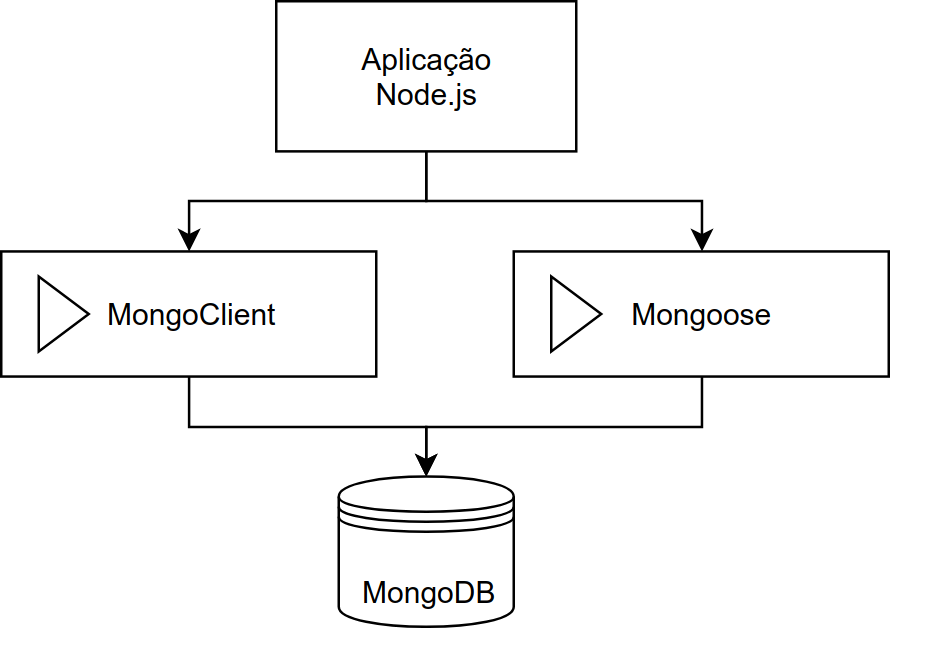
\includegraphics[width=0.6\textwidth]{images/diagram-banco}
    \label{fig:diagrama-banco}
\end{figure}


\textbf{Q1} --~\emph{O tamanho médio dos registros impacta de modo relevantes quanto ao uso de memória nas operações de CRUD?}

\textbf{Q2} -- O tamanho médio dos registros pode influenciar no uso de CPU nas operações de CRUD? 

\textbf{Q3} -- O tamanho médio dos registros impacta no tempo de execução de cada uma das operações de CRUD?


\subsection{Dataset}

O presente estudo utilizou um conjunto de dados com cerca 18 mil instâncias de dados, proveniente do seguinte dataset~\footnote{https://www.kaggle.com/karangadiya/fifa19}.
Originalmente, todos os registros presentes são compostos por 89 atributos, predominante textuais, obtendo um tamanho médio de 1,37KB.
A partir do conjunto original, foi construído um conjunto reduzido em número de atributos (6 atributos), com o mesmo total de instância, porém com tamanho médio de 0,13KB.


\subsection{Ambiente de Execução}

O ambiente de execução para os testes de desempenho consistiu em um computador pessoal com sistema operacional Ubuntu 18.04.2, processador Intel i3 3217U e memória RAM de 5GB. 

Durante a execução dos testes, o ambiente de execução da aplicação Node.js foi definido o uso do~\emph{heap} de memória com limite máximo de 3GB, o que restringiu no limite superior do número de operações executadas em cada cenário de teste.

Em cada cenário de execução, foram extraídos dados relativos ao tempo de execução, tempo de uso de CPU e uso de memória RAM.
Foram analisados cenários com diferentes quantidades de operações CRUD realizadas, as quais variaram de 1000, 10000, 100000 e 200000; cada qual foi repetido 10 vezes. 

\subsection{Resultados}
\label{section:resultados}


Esses são os resultados de tempo
\begin{figure*}
  \centering
  \begin{subfigure}[b]{0.48\textwidth}
    \centering
    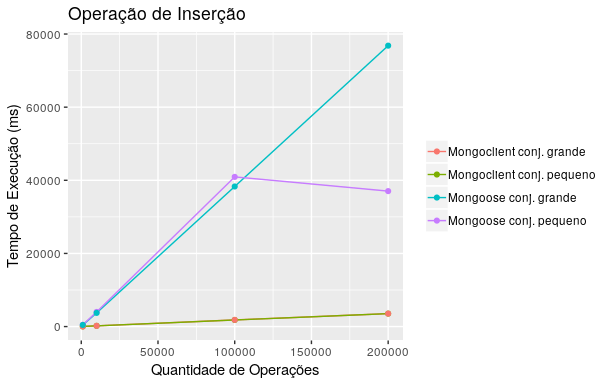
\includegraphics[width=\textwidth]{images/difftime-create-pt}
    \label{fig:difftime-a}
  \end{subfigure}
  \hfill
  \begin{subfigure}[b]{0.48\textwidth}  
    \centering 
    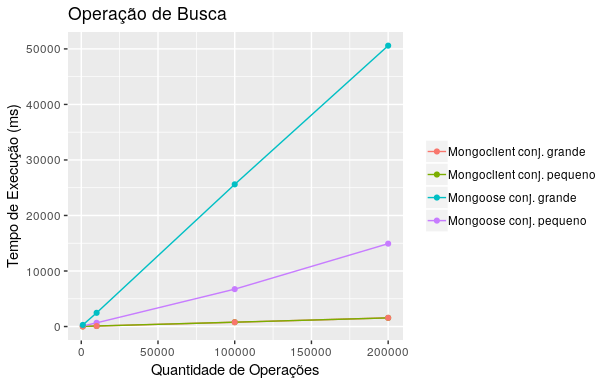
\includegraphics[width=\textwidth]{images/difftime-read-pt}
    \label{fig:difftime-b}
  \end{subfigure}
  \vskip\baselineskip
  \begin{subfigure}[b]{0.48\textwidth}   
    \centering 
    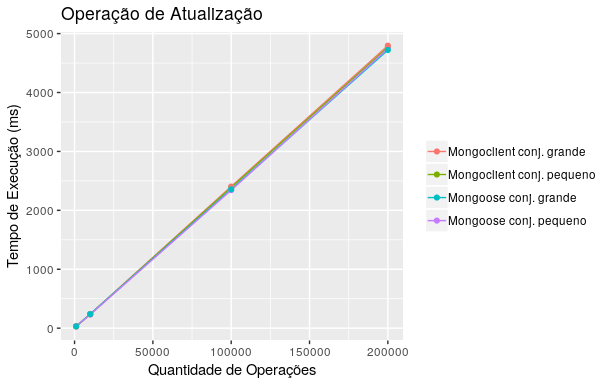
\includegraphics[width=\textwidth]{images/difftime-update-pt}   
    \label{fig:difftime-c}
  \end{subfigure}
  \quad
  \begin{subfigure}[b]{0.48\textwidth}   
    \centering 
    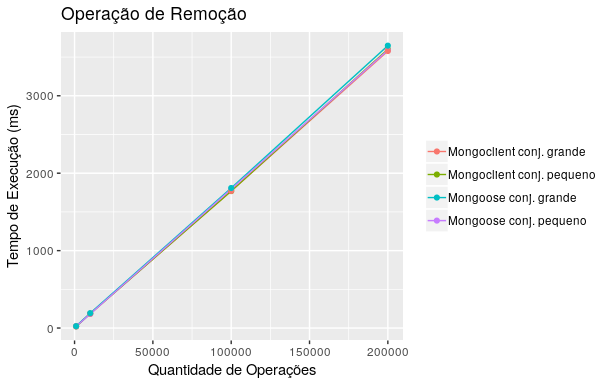
\includegraphics[width=\textwidth]{images/difftime-delete-pt}  
    \label{fig:difftime-d}
  \end{subfigure}
  \caption{ The average and standard deviation of critical parameters}
\label{fig:diff-geral}
\end{figure*}


Esses são os resultados de uso de cpu
\begin{figure*}
  \centering
  \begin{subfigure}[b]{0.48\textwidth}
    \centering
    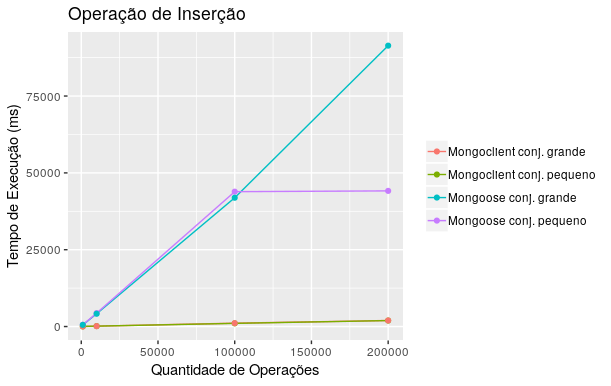
\includegraphics[width=\textwidth]{images/cpuusage-create-pt}
    \label{fig:cpuusage-a}
  \end{subfigure}
  \hfill
  \begin{subfigure}[b]{0.48\textwidth}  
    \centering 
    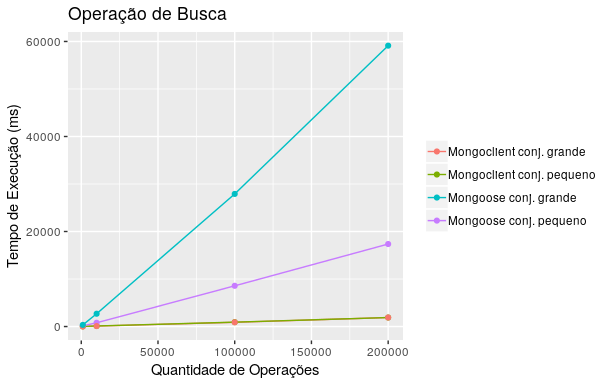
\includegraphics[width=\textwidth]{images/cpuusage-read-pt}
    \label{fig:cpuusage-b}
  \end{subfigure}
  \vskip\baselineskip
  \begin{subfigure}[b]{0.48\textwidth}   
    \centering 
    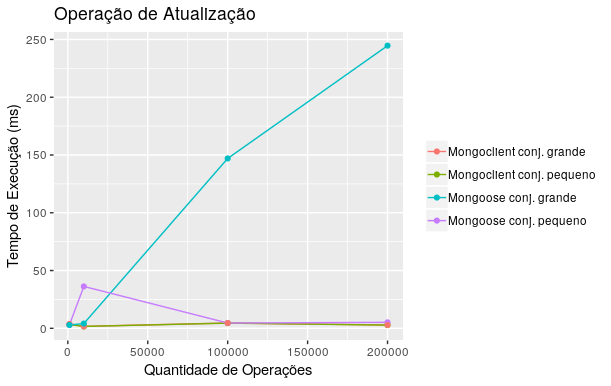
\includegraphics[width=\textwidth]{images/cpuusage-update-pt}   
    \label{fig:cpuusage-c}
  \end{subfigure}
  \quad
  \begin{subfigure}[b]{0.48\textwidth}   
    \centering 
    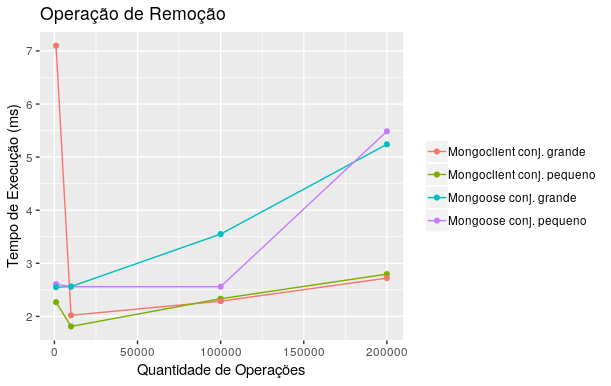
\includegraphics[width=\textwidth]{images/cpuusage-delete-pt}  
    \label{fig:cpuusage-d}
  \end{subfigure}
  \caption{ The average and standard deviation of critical parameters}
\label{fig:cpuusage-geral}
\end{figure*}


Esses são os resultados de uso de memoria
\begin{figure*}
  \centering
  \begin{subfigure}[b]{0.48\textwidth}
    \centering
    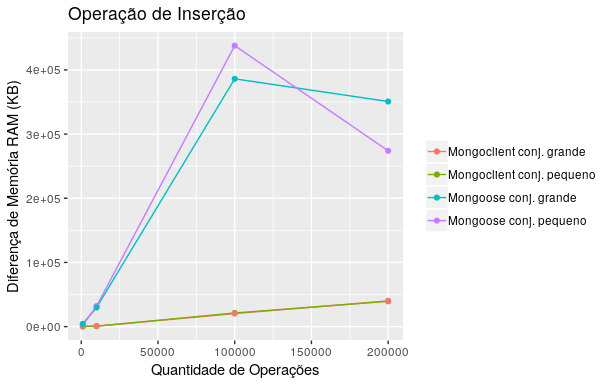
\includegraphics[width=\textwidth]{images/memory-create-pt}
    \label{fig:memory-a}
  \end{subfigure}
  \hfill
  \begin{subfigure}[b]{0.48\textwidth}  
    \centering 
    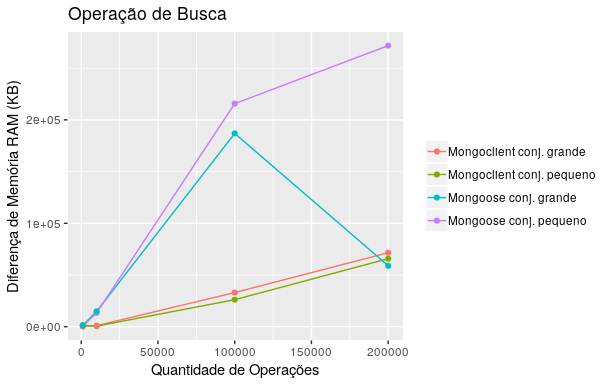
\includegraphics[width=\textwidth]{images/memory-read-pt}
    \label{fig:memory-b}
  \end{subfigure}
  \vskip\baselineskip
  \begin{subfigure}[b]{0.48\textwidth}   
    \centering 
    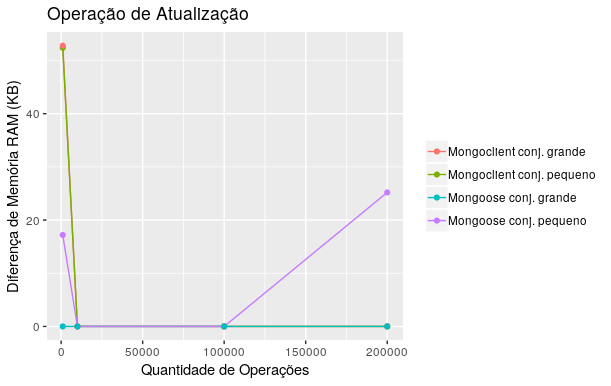
\includegraphics[width=\textwidth]{images/memory-update-pt}   
    \label{fig:memory-c}
  \end{subfigure}
  \quad
  \begin{subfigure}[b]{0.48\textwidth}   
    \centering 
    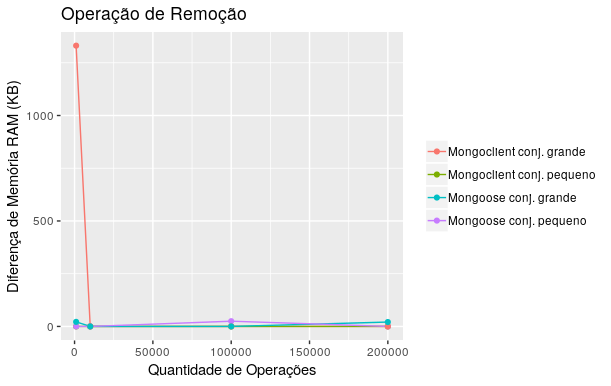
\includegraphics[width=\textwidth]{images/memory-delete-pt}  
    \label{fig:memory-d}
  \end{subfigure}
  \caption{ The average and standard deviation of critical parameters}
\label{fig:memory-geral}
\end{figure*}



\section{Discussão dos Resultados}
\label{section:discussao}

\subsection{Discussão da Q1}

\subsection{Discussão da Q2}

\subsection{Discussão da Q3}


\section{Ameaças à Validação}
\label{section:limitacoes}



\section{Trabalhos Relacionados} 
\label{section:relacionados}

The first page must display the paper title, the name and address of the
authors, the abstract in English and ``resumo'' in Portuguese (``resumos'' are
required only for papers written in Portuguese). The title must be centered
over the whole page, in 16 point boldface font and with 12 points of space
before itself. Author names must be centered in 12 point font, bold, all of
them disposed in the same line, separated by commas and with 12 points of
space after the title. Addresses must be centered in 12 point font, also with
12 points of space after the authors' names. E-mail addresses should be
written using font Courier New, 10 point nominal size, with 6 points of space
before and 6 points of space after.

The abstract and ``resumo'' (if is the case) must be in 12 point Times font,
indented 0.8cm on both sides. The word \textbf{Abstract} and \textbf{Resumo},
should be written in boldface and must precede the text.


\section{Considerações Finais}
\label{section:consideracoes}

\section{Referências Bibliográficas}

\bibliographystyle{sbc}
\bibliography{sbc-template}

\end{document}
